\chapter{СБОР ОБУЧАЮЩИХ ДАННЫХ} \label{chapt3}{}

Для решения задачи классификации нейронной сетью требуется наличие данных для обучения. Датасетов с настоящей задачей в открытом доступе не нашлось, поэтому данные пришлось получать вручную. Процесс сбора данных, описанный здесь, идентичен описанному в авторской статье \cite{dogo}.

\begin{figure}[ht] 
  \center
  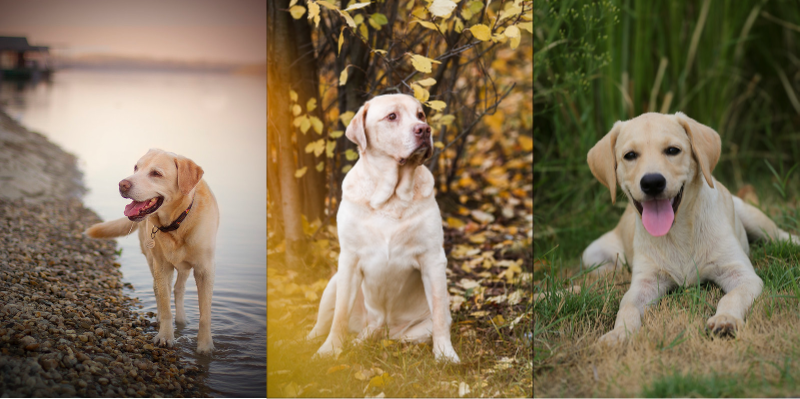
\includegraphics [width=\textwidth*2/3] {dogs-classes}
  \caption{Позы собаки, на которые классифицируются изображения: собака стоит, собака сидит и собака лежит} 
  \label{img:classes}  
\end{figure}

За основу был взят датасет OpenImageDataset\cite{openimages} - набор изображений на более чем тысячу разных классов. Из него был взят подкласс Dog, в котором было 20000 изображений собак. Далее эти данные были размечены на Яндекс.Толоке. 

Каждое изображение было показано пользователю Толоки с вопросом “В какой позиции собака находится на этом фото”. Пример таких поз виден на рисунке \ref{img:classes}. Фотографии были размечены с пятикратным перекрытием, т.е. каждое изображение размечалось пять раз разными людьми. На выходе получился скромного размера датасет, часть изображений в нём не подходили под постановку задач, но на выходе имелась информация о позе собаки, а также об ограничивающей рамке конечностей, с уклоном в будущее.

Перед тем, как загружать данные в нейронную сеть, они были предобработаны. Вместе с комплектом данных из OpenImageDataset шла таблица с информацией о следующем:
\begin{itemize}[wide]
    \item Координаты ограничивающей рамки объекта;
    \item Список объектов в кадре;
    \item Флаг того, что объект загорожен;
    \item Флаг того, что объект обрезан;
    \item Флаг того, что объект - рисунок объекта, а не фотография;
    \item Флаг того, что объект является группой объектов;
    \item Флаг того, что объект находится внутри другого объекта.
\end{itemize}
В идеальном случае, все флаги должны быть равны нулю - то есть объект не загорожен, не обрезан и не рисунок. Но если применить все фильтры, окажется что из 20000 изображений осталось всего 5000. При этом оказалось так, что флагами может быть отсеяно много годных изображений, но при этом могут остаться и обрезанные, и загороженные изображения собак. Это совсем неконсистентный результат. А вот ограничивающая рамка действительно может помочь. Пример такого изображения на рисунке \ref{img:crop_helps}.

\begin{figure}[ht] 
  \center
  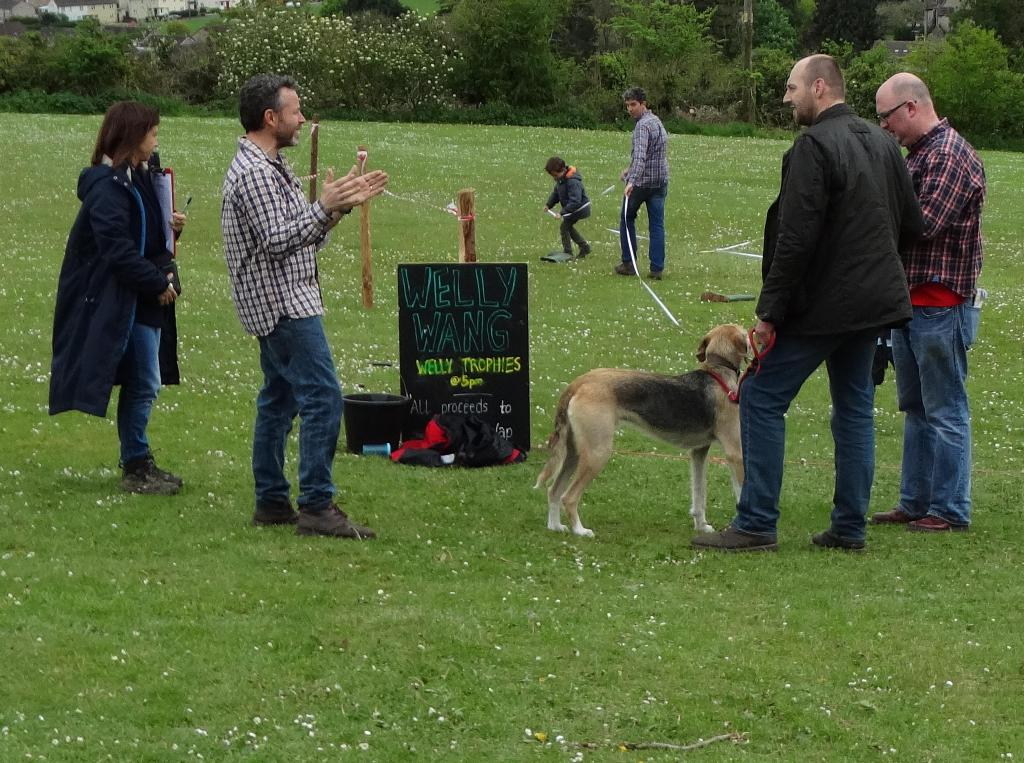
\includegraphics [width=\textwidth*2/3] {crop_helps}
  \caption{Изображение, которому сильно помогло бы обрезание по ограничивающей рамке собаки} 
  \label{img:crop_helps}  
\end{figure}

Хотя свёрточные нейронные сети инвариантны к расположению объектов в кадре, они сохраняют зависимость к отвлекающим объектам в кадре. Поэтому на практике обрезание изображения по ограничивающей рамке собаки помогает значительно ускорить процесс обучения нейронной сети и сделать его более стабильным. К тому же, это частично избавляет  от множественных собак в кадре, как на рисунке \ref{img:crop_helps} .

В итоге были предприняты следующие меры для улучшения работы системы.
\begin{itemize}[wide]
    \item Все изображения были обрезаны по ограничивающей рамке собаки. И это дало сильный прирост в качестве классификации, $55\% \rightarrow 65\%$ на 5 классах;
    \item Дополнительно были размечены и были удалены из выборки изображения, где собака видна плохо. Это сократило размер и без того маленькой выборки, не сильно улучшив данные, т.к. качество разметки на Толоке достаточно низкое;
    \item Добавлены аугментации обучающей выборки. Аугментации позволяют нейронной сети не запоминать обучающие данные точь-в-точь, что снижает её способность к переобучению;
    \item Проведена очистка изображений. Из обучающей выборки были исключены изображения с несколькими собаками и собаками, которых не видно целиком. Это дало самый ощутимый прирост, но обучающая выборка сократилась до недопустимо маленьких размеров. Добавлено около 3\% точности, $67\% \rightarrow 69\%$;
    \item Использование transfer learning (переносимость обучения) - все модели, которые использовались здесь, не обучались с нуля. Они обучались на нейронной сети, уже предобученной классифицировать 1000 классов ImageNet(другого открытого датасета с изображениями).
\end{itemize}

\section{Создание эталонного мини-датасета} \label{subsect3_1_2}
Датасет из OpenImageDataset обладал рядом недостатков. Вне зависимости от того каким фильтром выбирались из него данные, и как бы изображения не вырезались, с любой глубиной нейронной сети не выбиралась, нейронные сети не могли понять по этому датасету задачу и не показывали надёжное качество. Более того, из-за сильного дисбаланса классов некоторые категории игнорировались классификатором в пользу более популярных. Для сравнения, в категории ''собака лежит на спине''  насчитывалось всего 400 изображений, против 4500 у категории стоящих собак.

Поэтому, учитывая прошлые ошибки, было принято решение собрать датасет заново, используя опыт, полученный при разметке первого.

Главные изменения заключаются в следующем:
\begin{itemize}[wide]
    \item Датасет собирается итеративно по небольшим частям и выводы делаются сразу
    \item Размер каждого класса удерживается на одинаковом уровне
    \item Проводится учёт всех изображений, которые тяжело размечать
\end{itemize}{}

В статье Amy Bearman и Cathering Dong \cite{Bearman2015HumanPE} указывается, что нейронным сетям тяжело распознать позу, при наличии окклюзий, поворотов и переворотов, сильных перспективных искажений, и множественных объектов. Они представлены на рисунке \ref{img:hazards_dogs}. В новом датасете было уделено особое внимание трудноклассифицируемым изображениям, поэтому они всячески избегались.

\begin{figure}[ht] 
  \center
  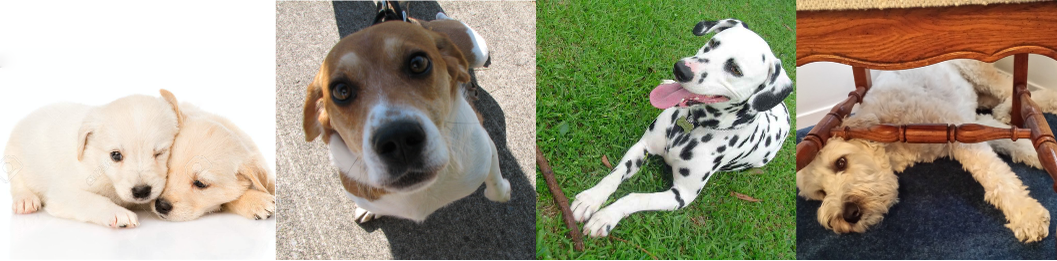
\includegraphics [width=\textwidth] {hazards_dogs}
  \caption{Позы, которые трудно определить: множественные объекты, перспективные искажения, повороты и окклюзии} 
  \label{img:hazards_dogs}  
\end{figure}

На этот раз источником изображений был Flickr. В нём содержится множество фотографий, которые можно было фильтровать
\begin{itemize}[wide]
    \item по ориентации - например, только вертикальные;
    \item по породе - можно явно указать, что мы ищем лабрадора ретривера;
    \item только снятые на телефон.
\end{itemize}

Собирать фотографии заново было достаточно хорошим упражнением, но главной проблемой были огромные временные затраты на создание датасета даже с 300 фотографиями. Более того, из 80000 фотографий по тегу \textit{лабрадор ретривер} автором и его ассистентом было просмотрено 70000 из них. И уже из них были собраны 300 фотографий, по 100 изображений на целевой класс. 

\section{Разметка данных нейронной сетью} \label{nn_labeling}
Нейронная сеть может сильно помогать в разметке данных. Порой, даже экономя время разметчиков в несколько раз. Главная идея в том, что искать ошибки классификации нейронной сети намного проще, чем размечать данные самому. 
В наличии имелись следующие данные:
\begin{itemize}[wide]
    \item датасет с собаками одной породы по 100 изображений на класс
    \item повторно размеченные, "наиболее удачные";
    \footnote{Фотографии, на которых собака одна, и её ничто не загораживает} 
    5000 фотографий из 20000 доступных в OpenImageDataset;
    \item все изображения с классом Dog в OpenImageDataset (их 20000, они не размечены).
\end{itemize}


Также была нейронная сеть, которая с 76\% точностью определяла, сидят собаки, лежат или стоят. Такая точность не подойдёт для итогового продукта, но даже её достаточно, чтобы узнать у самой нейронной сети, какие фотографии ей легко различать, а какие нет.

Проклассифицировав весь датасет, были выбраны только изображения, в которых нейронная сеть не ошиблась, и уверенность была выше 99\%. Таких изображений из 5000 оказалось всего 400, причём 250 из них были те, где собака стоит. И всего 40, где собака сидит. 

Это очень сильный дисбаланс. Но зато можно гарантировать что все картинки, которые попали в этот крошечный датасет будут легко классифицироваться нейросетью. Примеры из этого датасета показаны на рисунках \ref{img:laying_perfect_dogs} , \ref{img:perfectly_sitting}  и \ref{img:perfect_standing}.

% и здесь три подборки этих изображений по 20 штук на класс.

\begin{figure}[ht] 
  \center
  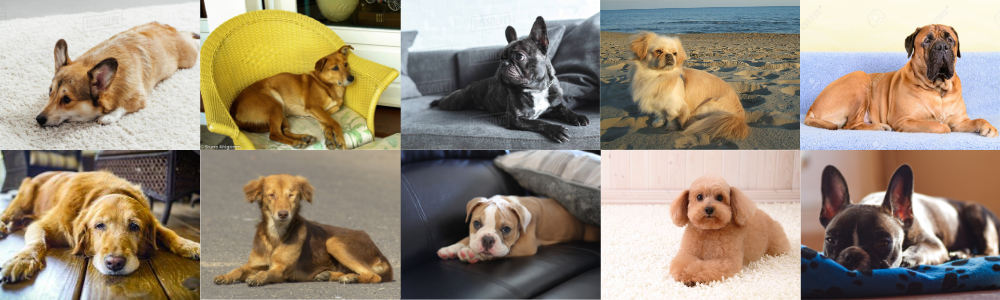
\includegraphics [width=\textwidth] {laying_perfect_dogs}
  \caption{Образец эталона лежащих собак из датасета} 
  \label{img:laying_perfect_dogs}  
\end{figure}

\begin{figure}[t] 
  \center
  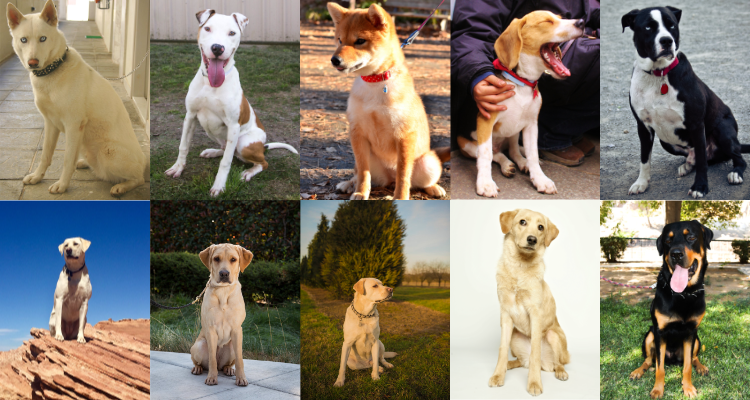
\includegraphics [width=\textwidth] {perfectly_sitting}
  \caption{Образец эталона сидячих собак из датасета} 
  \label{img:perfectly_sitting}  
\end{figure}

\begin{figure}[ht] 
  \center
  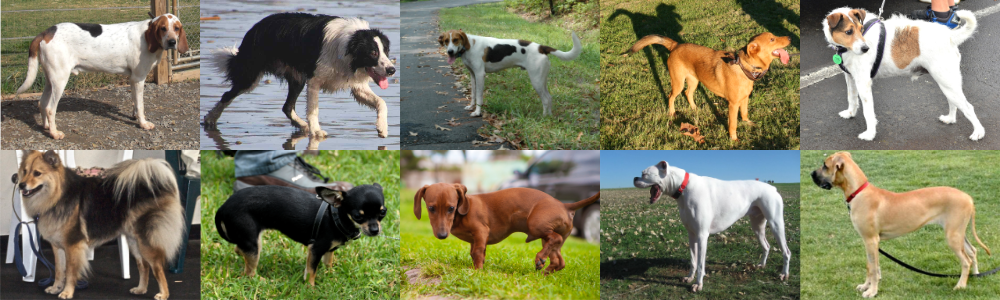
\includegraphics [width=\textwidth] {perfect_standing}
  \caption{Образец эталона стоящих собак из датасета} 
  \label{img:perfect_standing}  
\end{figure}


 Все собаки в этом новом датасете на достаточном отдалении от камеры и все их конечности хорошо видны, т.е. не загораживают друг друга.

\section{Получение датасета}\label{acq_dataset}

На основе увиденного было принято решение собрать по этим эталонам больше собак, хотя бы по 500 на класс. В дальнейшем оказалось, что уверенность нейронной сети -- относительный параметр. Классы, которые нейронная сеть легко классифицирует, обладают достаточной дисперсией вокруг 100\% вероятности. На практике это означало, что для хорошо подготовленного класса сидячих собак, можно было опустить уверенность сети до 93\%, чтобы иметь схожую вероятность получить эталонные кадры.

Каждый класс датасета был дополнен лучшими его представителями до одинакового количества изображений на класс. После этого изображения прошли дополнительную чистку на наличие спорных изображений, как на рисунке \ref{img:in_between}. Это позволило поднять количество изображений до, примерно, 300 на класс.

% спорное изображение, не понятно собака стоит или сидит.
\begin{figure}[ht] 
  \center
  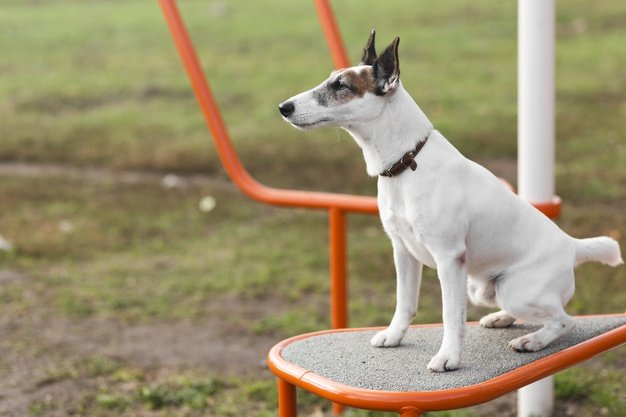
\includegraphics [width=\textwidth*2/3] {sit_or_stand}
  \caption{Спорное изображение. Не понятно, собака стоит или сидит.} 
  \label{img:in_between}  
\end{figure}

Окончательно поставить точку в количестве данных позволил всё тот же, плохо размеченный OpenImageDataset. В нём все 20000 изображений были отклассифицированы, и лучшие его представители тоже были отобраны, а затем вручную проверены. В итоге это позволило добавить ещё по 200 изображений на класс до общих 500. 
Получается, выход достаточно небольшой: из 20000 изображений, частью нового датасета стали всего лишь 1500. (Напомним, что предыдущие изображения были тоже взяты из этого датасета).
Недостающие изображения сидячих собак были дополнены 100 фотографиями сидячих лабрадоров из flickr. 

Маленький сет практически идеален, поэтому его можно брать без дополнительной проверки.

\section{Расширение датасета}\label{expanding_dataset}
Работать с маленькими датасетами на больших нейронных сетях крайне тяжело. Конечно, предобучение нейронных сетей на крупных наборах данных, таких как ImageNet, сильно помогает обучить глубокие слои и улучшает стабильность обучения, но 1500 изображений, порой, может не хватить даже для обучения «головы» нейронной сети.

Поэтому датасет постепенно расширялся в объёме по схожему принципу, указанному в предыдущей главе. На этот раз источником изображений стала группа «Shiba Inu Photography» в Facebook. В главном альбоме группы содержится 120 тысяч изображений, загруженных владельцами собак породы Шиба Ину.

Из загруженных 20000 изображений в датасет попало 2205 изображений. То есть, как и изначально, всего 1 изображение из 10 оригинальных попадает в конечный датасет.

Итоговое количество изображений стало уже по 1500 изображений на класс, то есть 4500 изображений. Это уже сравнимо с часто используемыми датасетами как Animal Image Dataset(DOG, CAT and PANDA), в котором содержится по 1000 изображений собак, котов и панд. 


\section*{Выводы по разделу 3}
\addcontentsline{toc}{section}{Выводы по разделу 3}
Был проведён анализ ошибок и выявлены следующие:
\begin{enumerate}[wide, labelwidth=!, labelindent=1.25cm]
    \item Для разметки данных надо использовать постоянных сотрудников, которым надо уделить время на то, чтобы разобраться с задачей. Низкая цена обучения не компенсирует многократные перекрытия, в надежде найти статистическое среднее;
    \item Количество весов в нейронной сети и количество изображений в датасете должны быть линейно связаны. Хороший размер обучающей выборки для ResNet-34 (2.4 миллиона параметров) - строго от 100 тысяч изображений;
    \item Датасет надо балансировать по количеству изображений в каждом классе;
    \item В данных была огромная внутриклассовая разница между изображениями. У собак множество пород и размеров. Так как точность разметки не идеальна, нейронная сеть может запомнить, что собака сидит, когда она чёрная, например. 
\end{enumerate}{}



\textit{Достоинства полученного датасета:}
\begin{enumerate}[wide, labelwidth=!, labelindent=1.25cm]
    \item Есть датасет, на котором принципиально возможно обучить нейронную сеть;
    \item Точность классификации достаточна для поставленной задачи;
    \item Создан способ, позволяющий получить датасет любого размера. Требуется только однократная валидация человеком.
\end{enumerate}


\textit{Недостатки полученного датасета:}
\begin{enumerate}[wide, labelwidth=!, labelindent=1.25cm]
    \item Нейронная сеть в состоянии работать только при удовлетворении некоторых условий;
    \item Датасет не предусматривает наличие пограничных случаев, например, когда собака сидит, но не совсем обычным образом - не все позы собаки можно поделить на "сидит", "стоит" и "лежит".
\end{enumerate}

Собаки часто лежат на спине, на боку, лежат с поднятой головой и т.д. Собаки ещё бегут, прыгают и кружатся. Все эти случаи не попадают под нашу классификацию.


Теперь при наличии подходящего датасета, можно приступить к решению задачи по разработке самой системы по определению позы собак по видеопотоку.